\documentclass[a4paper,12pt]{article}
\usepackage{graphicx}
\graphicspath{{.}}

\usepackage{calc}
\setlength\textwidth{7in}
\setlength\textheight{10in}
\setlength\oddsidemargin{(\paperwidth-\textwidth)/2 - 1in}
\setlength\topmargin{(\paperheight-\textheight
	-\headheight-\headsep-\footskip)/2 - 1in}

\begin{document}

	
	\title{Tema Curs 8 Baze de Date}
	\author{Moroianu Theodor (135)}
	\date{\today}
	\maketitle

	\section{Creearea unor cereri SQL}
		\textit{Pentru exemplul de optimizare a unei cereri asupra modelului referitor la operele de arta, se cere codul SQL corespunzător arborelui inițial și arborelui optimizat. Diagrama și cerinta se află în fișierul Exemplu\_optimizare\_cerere\_opere\_arta.pdf, iar cei 2 arbori se află în fișierul arbori\_cerere\_opere\_arta.png.}\\
		\newline
		\begin{itemize}
			\item \textbf{Codul corespunzator diagramei ne-optimizate:}\\
			SELECT titlu, valoare\\
			FROM (SELECT o.cod\_opera, o.titlu, o.valoare\\
			FROM (SELECT *\\
			FROM colectie\\
			WHERE proprietar='VV') c\\
			JOIN\\
			(SELECT *\\
			FROM opera\\
			WHERE cod\_calerie='G1') o\\
			ON (c.opera=o.opera))\\
			\\
			INTERSECT\\
			\\
			(SELECT w.cod\_opera, w.titlu, w.valoare\\
			FROM (SELECT cod\_opera\\
			FROM restaureaza\\
			WHERE data$>$'15-JUN-2000') r\\
			JOIN\\
			(SELECT cod\_opera, titlu, valoare\\
			FROM opera) w\\
			ON (w.cod\_opera=r.cod\_opera))\\
			
			\item \textbf{Codul corespunzator diagramei optimizate:}\\
			
			SELECT g.titlu, g.valoare\\
			FROM (SELECT cod\_opera\\
			FROM restaureaza\\
			WHERE data$>$'15-JUN-2000') r\\
			JOIN\\
			(SELECT o.cod\_opera, o.titlu, o.valoare, o.cod\_colectie\\
			FROM opera o JOIN colectie c ON(o.cod\_opera=c.cod\_opera)\\
			WHERE cod\_galerie='G1' AND c.proprietar='VV') g\\
			ON (r.cod\_opera=g.cod\_opera)\\
			
		\end{itemize}
	
	\section{Gestiunea unei platforme de e-learning: diagrama conceptuală, scheme relaționale}
		
		\textbf{Schema Relationala:}
		
		\begin{itemize}
			\item Grupa(\#ID\_grupa, an, numar\_elevi)
			\item Orar(\#ID\_orar, curs, zi\_si\_ora\_curs, data\_examen, semestru, grupa)
			\item Cursuri(\#ID\_curs, nume, profesor)
			\item Studenti(\#ID\_student, nume, grupa, varsta)
			\item Note(\#ID\_nota, curs, student, nota)
			\item Profesori(\#ID\_profesor, nume\_profesor, prenume\_profesor, grad\_didactic)
			\item Materiale(\#ID\_material, curs, tip\_material, link, student)
		\end{itemize}
	
		\textbf{Diagrama Conceptuala:}
		
		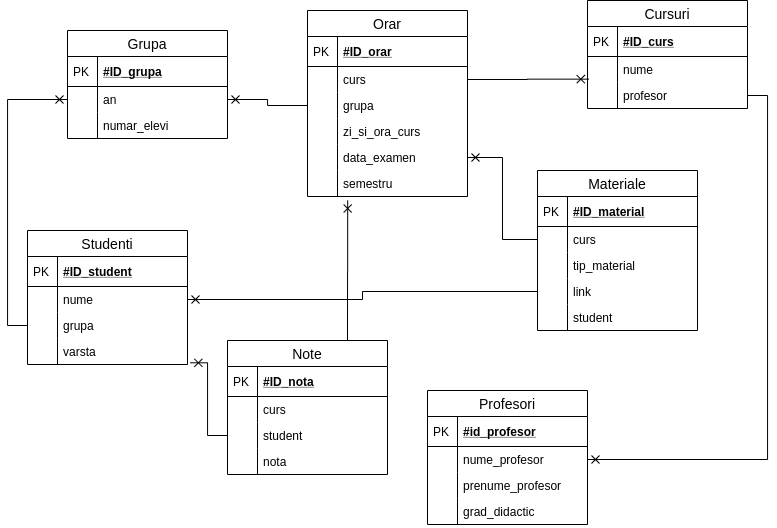
\includegraphics[scale=0.6]{BDTemaCurs8DiagramaConceptuala.png}
		\newpage
		
		
		\textbf{Cereri SQL:}
		
		\begin{itemize}
			\item Cursurile la care sunt inrolati studentii\\
			\textit{
			SELECT UNIQUE o.cursuri\\
			FROM studenti s JOIN orar o ON (s.grupa=o.grupa)\\
			WHERE o.semestru='2020/1';}
			
			\item Care sunt materialele (documente, link-uri externe etc) de curs/laborator/seminar care vizează un anumit student, pentru un anumit curs?
			
			\textit{SELECT link\\
				FROM materiale\\
				WHERE curs=\&curs AND student=\&student;}
			\item 
			Care sunt notele studenților la materiile studiate?
			
			\textit{SELECT nota, curs, student\\
			FROM note;}
			\item Când au loc sesiunile online de curs sau examinare? \\
			\textit{
			SELECT data\_examen, grupa, curs\\
			FROM orar;}
				
		\end{itemize}
		
	
	
\end{document}















